% =====================================================================
%  TEMPLATE Artikel Prosiding / Jurnal Teknik ITS (gaya POMITS)
% ---------------------------------------------------------------------
%  Sumber LaTeX ini DIKONVERSI ke .docx dengan Pandoc (lihat build-docx.ps1).
%  Styling (font TNR, heading, A4, 2 kolom) diatur lewat reference.docx.
%  Persamaan -> OMML (equation Word), \textit -> miring, _{} -> subskrip.
%
%  Build:   ./build-docx.ps1        (atau VSCode: Run Task "LaTeX to DOCX")
%
%  >>> YANG PERLU DIEDIT: bagian \title dan \author di bawah, lalu isi
%      naskah di folder bagian/. Cari penanda "TODO" di seluruh proyek.
% =====================================================================
\documentclass[11pt,a4paper]{article}
\usepackage[utf8]{inputenc}
\usepackage[T1]{fontenc}
\usepackage[indonesian]{babel}
\usepackage{graphicx}
\usepackage{amsmath,amssymb}
\usepackage{booktabs}
\usepackage{array}
\graphicspath{{gambar/}}

% TODO: Ganti judul artikel Anda. Ditulis ringkas & informatif (Title Case),
% Times New Roman 24pt non-bold rata tengah. Pakai \textit{...} untuk istilah asing.
\title{Judul Artikel Ilmiah Ditulis Ringkas, Jelas, dan Informatif
Menggunakan Huruf \textit{Title Case}}

% TODO: Ganti nama penulis, pembimbing, afiliasi, dan e-mail.
\author{Nama Penulis, Nama Pembimbing, dan Nama Ko-Pembimbing\\
Departemen Teknik XXXX, Fakultas XXXX\\
Institut Teknologi Sepuluh Nopember (ITS)\\
Jl. Arief Rahman Hakim, Surabaya 60111\\
e-mail: nrp@student.its.ac.id}
\date{}

\begin{document}
\maketitle

% Tiap bagian disimpan terpisah di folder bagian/ (rapi & expandable).
% Untuk menambah bagian: buat file baru lalu \input di bawah ini.
\input{bagian/00-abstrak}
% CONTOH (lorem ipsum). Huruf pertama paragraf pertama otomatis jadi drop cap.
\section{I. PENDAHULUAN}

Lorem ipsum dolor sit amet, consectetur adipiscing elit, sed do eiusmod tempor
incididunt ut labore et dolore magna aliqua \cite{ContohSatu2024}. Ut enim ad
minim veniam, quis nostrud exercitation ullamco laboris nisi ut aliquip ex ea
commodo consequat. Duis aute irure dolor in reprehenderit in voluptate velit
esse cillum dolore eu fugiat nulla pariatur, parameter $K_p$ dan $K_i$ tetap.
Excepteur sint occaecat cupidatat non proident, sunt in culpa qui officia
deserunt mollit anim id est laborum \cite{ContohDua2023}.

Sed ut perspiciatis unde omnis iste natus error sit voluptatem accusantium
doloremque laudantium, totam rem aperiam, eaque ipsa quae ab illo inventore
veritatis et quasi architecto beatae vitae dicta sunt explicabo
\cite{ContohSatu2024,ContohProsiding2022}. Nemo enim ipsam voluptatem quia
voluptas sit aspernatur aut odit aut fugit, sed quia consequuntur magni dolores
eos qui ratione \textit{voluptatem} sequi nesciunt. Neque porro quisquam est,
qui dolorem ipsum quia dolor sit amet, consectetur, adipisci velit.

Quis autem vel eum iure reprehenderit qui in ea voluptate velit esse quam nihil
molestiae consequatur, vel illum qui dolorem eum fugiat quo voluptas nulla
pariatur \cite{ContohBuku2011}. Berdasarkan hal tersebut, dua permasalahan
dirumuskan: (RM-1) at vero eos et accusamus et iusto odio dignissimos ducimus;
dan (RM-2) qui blanditiis praesentium voluptatum deleniti atque corrupti quos
dolores et quas molestias excepturi sint occaecati cupiditate non provident.

% CONTOH (lorem ipsum) — demonstrasi subbab, gambar, persamaan, dan tabel.
\section{II. URAIAN PENELITIAN}

\subsection{A. Rancangan Sistem}

Lorem ipsum dolor sit amet, consectetur adipiscing elit, sed do eiusmod tempor
incididunt ut labore et dolore magna aliqua. Ut enim ad minim veniam, quis
nostrud exercitation ullamco laboris nisi ut aliquip ex ea commodo consequat,
seperti diilustrasikan pada Gambar~1. Duis aute irure dolor in reprehenderit in
voluptate velit esse cillum dolore eu fugiat nulla pariatur.

\begin{figure}[h]
  \centering
  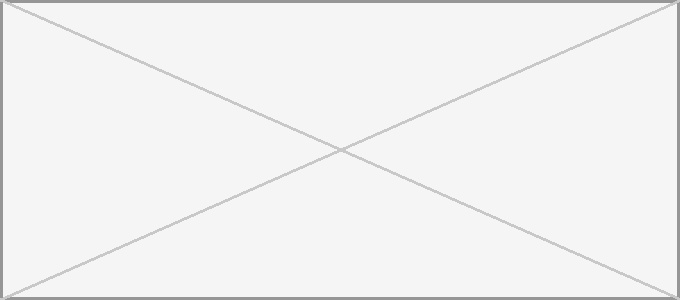
\includegraphics[width=8.5cm]{gambar/contoh-gambar.png}
  \caption{Gambar 1. Lorem ipsum dolor sit amet, consectetur adipiscing elit:
  keterangan gambar diletakkan di bawah gambar dan diberi nomor manual.}
\end{figure}

Lorem ipsum dolor sit amet, consectetur adipiscing elit, sed do eiusmod tempor
incididunt ut labore et dolore magna aliqua. Ut enim ad minim veniam, quis
nostrud exercitation ullamco laboris nisi ut aliquip ex ea commodo consequat
\cite{ContohProsiding2022}. Duis aute irure dolor in reprehenderit in voluptate
velit esse cillum dolore eu fugiat nulla pariatur. Excepteur sint occaecat
cupidatat non proident, sunt in culpa qui officia deserunt mollit anim id est
laborum \cite{ContohDua2023}.

\subsection{B. Model Matematis}

Sed ut perspiciatis unde omnis iste natus error sit voluptatem accusantium
doloremque laudantium. Hubungan masukan--keluaran dinyatakan pada (1), dengan
$K_p$ \textit{gain} proporsional dan $K_i$ \textit{gain} integral.
\begin{equation*}
  y(t) = K_p\,e(t) + K_i \int_{0}^{t} e(\tau)\, d\tau \qquad\text{(1)}
\end{equation*}
Totam rem aperiam, eaque ipsa quae ab illo inventore veritatis et quasi
architecto beatae vitae dicta sunt explicabo, sehingga diperoleh bentuk orde dua
baku pada (2).
\begin{equation*}
  G(s) = \frac{\omega_n^{2}}{s^{2} + 2\zeta\omega_n s + \omega_n^{2}}
  \qquad\text{(2)}
\end{equation*}
dengan $\zeta$ rasio redaman dan $\omega_n$ frekuensi natural.

Nemo enim ipsam voluptatem quia voluptas sit aspernatur aut odit aut fugit, sed
quia consequuntur magni dolores eos qui ratione voluptatem sequi nesciunt. Neque
porro quisquam est, qui dolorem ipsum quia dolor sit amet, consectetur, adipisci
velit \cite{ContohBuku2011}. Sed ut perspiciatis unde omnis iste natus error sit
voluptatem accusantium doloremque laudantium, totam rem aperiam \cite{ContohSatu2024}.

At vero eos et accusamus et iusto odio dignissimos ducimus qui blanditiis
praesentium voluptatum deleniti atque corrupti quos dolores et quas molestias
excepturi sint occaecati cupiditate non provident. Similique sunt in culpa qui
officia deserunt mollitia animi, id est laborum et dolorum fuga. Et harum quidem
rerum facilis est et expedita distinctio. Nam libero tempore, cum soluta nobis
est eligendi optio cumque nihil impedit quo minus id quod maxime placeat facere
possimus \cite{ContohDua2023}.

\subsection{C. Parameter Rancangan}

Nemo enim ipsam voluptatem quia voluptas sit aspernatur, dengan parameter utama
dirangkum pada Tabel~1.

\begin{table}[h]
  \caption{Tabel 1. Lorem ipsum: spesifikasi dan parameter rancangan.}
  \centering
  \begin{tabular}{ll}
  \hline
  \textbf{Parameter} & \textbf{Nilai} \\
  \hline
  Lorem ipsum dolor   & 750 W / 36 V \\
  Consectetur, $p$    & 4 \\
  Adipiscing elit     & 16 kHz \\
  Tempor incididunt   & 18 A \\
  Sed do eiusmod      & 0{,}312~$\Omega$ \\
  Labore et dolore    & 0{,}147~mH \\
  Magna aliqua        & 6.400 rad/s \\
  \hline
  \end{tabular}
\end{table}

Temporibus autem quibusdam et aut officiis debitis aut rerum necessitatibus
saepe eveniet ut et voluptates repudiandae sint et molestiae non recusandae
\cite{ContohProsiding2022}. Itaque earum rerum hic tenetur a sapiente delectus,
ut aut reiciendis voluptatibus maiores alias consequatur aut perferendis
doloribus asperiores repellat.

\subsection{D. Prosedur Pengujian}

Curabitur pretium tincidunt lacus. Nulla gravida orci a odio. Nullam varius,
turpis et commodo pharetra, est eros bibendum elit, nec luctus magna felis
sollicitudin mauris. Integer in mauris eu nibh euismod gravida. Duis ac tellus
et risus vulputate vehicula. Donec lobortis risus a elit. Matriks pengujian
dirangkum pada Tabel~2.

\begin{table}[h]
  \caption{Tabel 2. Lorem ipsum: matriks pengujian.}
  \centering
  \begin{tabular}{cccc}
  \hline
  \textbf{Kondisi} & \textbf{Level 1} & \textbf{Level 2} & \textbf{Level 3} \\
  \hline
  Lorem   & 100 & 200 & 300 \\
  Ipsum   & 150 & 250 & 350 \\
  Dolor   & 200 & 300 & 400 \\
  Sit     & 250 & 350 & 450 \\
  Amet    & 300 & 400 & 500 \\
  \hline
  \end{tabular}
\end{table}

Etiam tempor. Ut ullamcorper, ligula eu tempor congue, eros est euismod turpis,
id tincidunt sapien risus a quam. Maecenas fermentum consequat mi. Donec
fermentum. Pellentesque malesuada nulla a mi \cite{ContohSatu2024}. Duis sapien
sem, aliquet nec, commodo eget, consequat quis, neque. Aliquam faucibus, elit ut
dictum aliquet, felis nisl adipiscing sapien, sed malesuada diam lacus eget
erat \cite{ContohBuku2011}. Cras mollis scelerisque nunc. Nullam arcu. Aliquam
consequat. Curabitur augue lorem, dapibus quis, laoreet et, pretium ac, nisi.

Fusce convallis, mauris imperdiet gravida bibendum, nisl turpis suscipit mauris,
sed placerat ipsum urna sed risus. In convallis tellus a mauris. Curabitur non
elit ut libero tristique sodales. Mauris a lacus. Donec mattis semper leo.
Vivamus facilisis diam at odio. Mauris dictum, nisi eget consequat elementum,
lacus ligula molestie metus, non fermentum dolor elit a nisl \cite{ContohDua2023}.
Quisque facilisis quam in odio. Nullam ornare quam in nulla.

\lipsum[6-12]

% CONTOH (lorem ipsum) — demonstrasi tabel hasil + gambar grafik.
\section{III. HASIL DAN DISKUSI}

\subsection{A. Hasil Pengujian}

Lorem ipsum dolor sit amet, consectetur adipiscing elit. Hasil pengujian
dirangkum pada Tabel~3, dengan baris tebal menandai nilai terpilih. Sed do
eiusmod tempor incididunt ut labore et dolore magna aliqua, ut enim ad minim
veniam quis nostrud exercitation.

\begin{table}[h]
  \caption{Tabel 3. Lorem ipsum: hasil pengujian (baris tebal = terpilih).}
  \centering
  \begin{tabular}{cccc}
  \hline
  \textbf{Kondisi} & \textbf{Metrik A} & \textbf{Metrik B} & \textbf{Metrik C} \\
  \hline
  Lorem   & 12{,}3  & 4{,}5  & 67{,}8 \\
  \textbf{Ipsum} & \textbf{8{,}7}  & \textbf{2{,}9}  & \textbf{42{,}3} \\
  Dolor   & 14{,}1  & 5{,}8  & 71{,}6 \\
  Sit     & 10{,}5  & 3{,}4  & 58{,}2 \\
  Amet    & 15{,}8  & 6{,}1  & 79{,}4 \\
  Elit    & 9{,}2   & 2{,}7  & 38{,}9 \\
  \hline
  \end{tabular}
\end{table}

Duis aute irure dolor in reprehenderit in voluptate velit esse cillum dolore eu
fugiat nulla pariatur. Excepteur sint occaecat cupidatat non proident, sunt in
culpa qui officia deserunt mollit anim id est laborum. Sed ut perspiciatis unde
omnis iste natus error sit voluptatem accusantium doloremque laudantium
\cite{ContohSatu2024}.

\subsection{B. Perbandingan Kinerja}

Ut enim ad minim veniam, quis nostrud exercitation ullamco laboris nisi ut
aliquip ex ea commodo consequat. Hasil perbandingan disajikan pada Tabel~4.

\begin{table}[h]
  \caption{Tabel 4. Lorem ipsum: persentase perbaikan.}
  \centering
  \begin{tabular}{>{\centering\arraybackslash}p{2.2cm}>{\centering\arraybackslash}p{1.0cm}cccc}
  \hline
  \textbf{Kolom1} & \textbf{Kolom2} & \multicolumn{4}{c}{\textbf{Header Grup}} \\
  & & \textbf{Sub1} & \textbf{Sub2} & \textbf{Sub3} & \textbf{Sub4} \\
  \hline
  A & X & +14\% & +19\% & +26\% & +31\% \\
  A & Y & +8\%  & +22\% & +17\% & +35\% \\
  A & Z & +21\% & +11\% & +33\% & +24\% \\
  B & X & +16\% & +28\% & +19\% & +38\% \\
  B & Y & +11\% & +13\% & +29\% & +22\% \\
  B & Z & +23\% & +18\% & +34\% & +41\% \\
  C & X & +9\%  & +25\% & +15\% & +36\% \\
  C & Y & +18\% & +14\% & +27\% & +20\% \\
  C & Z & +27\% & +32\% & +39\% & +44\% \\
  \hline
  \textbf{Rata-rata} & & \textbf{+16\%} & \textbf{+20\%} & \textbf{+27\%} & \textbf{+32\%} \\
  \hline
  \end{tabular}
\end{table}

Sed ut perspiciatis unde omnis iste natus error sit voluptatem accusantium
doloremque laudantium, totam rem aperiam, eaque ipsa quae ab illo inventore
veritatis et quasi architecto beatae vitae dicta sunt explicabo
\cite{ContohSatu2024,ContohDua2023}. Nemo enim ipsam voluptatem quia voluptas
sit aspernatur aut odit aut fugit, sed quia consequuntur magni dolores eos qui
ratione voluptatem sequi nesciunt.

\subsection{C. Pembahasan}

Ut enim ad minim veniam, quis nostrud exercitation ullamco laboris nisi ut
aliquip ex ea commodo consequat, sebagaimana tampak pada Gambar~2. Duis aute
irure dolor in reprehenderit in voluptate velit esse cillum dolore eu fugiat
nulla pariatur. Excepteur sint occaecat cupidatat non proident, sunt in culpa
qui officia deserunt mollit anim id est laborum \cite{ContohDua2023}.

\begin{figure}[h]
  \centering
  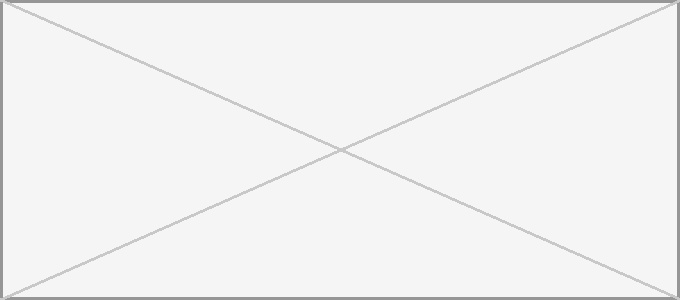
\includegraphics[width=8.5cm]{gambar/contoh-gambar.png}
  \caption{Gambar 2. Lorem ipsum dolor sit amet, consectetur adipiscing elit:
  contoh grafik hasil pengujian.}
\end{figure}

At vero eos et accusamus et iusto odio dignissimos ducimus qui blanditiis
praesentium voluptatum deleniti atque corrupti quos dolores et quas molestias
excepturi sint occaecati cupiditate non provident. Similique sunt in culpa qui
officia deserunt mollitia animi, id est laborum et dolorum fuga
\cite{ContohProsiding2022}. Et harum quidem rerum facilis est et expedita
distinctio. Nam libero tempore, cum soluta nobis est eligendi optio cumque nihil
impedit quo minus id quod maxime placeat facere possimus, omnis voluptas
assumenda est, omnis dolor repellendus \cite{ContohBuku2011}.

Temporibus autem quibusdam et aut officiis debitis aut rerum necessitatibus
saepe eveniet ut et voluptates repudiandae sint et molestiae non recusandae.
Itaque earum rerum hic tenetur a sapiente delectus, ut aut reiciendis
voluptatibus maiores alias consequatur aut perferendis doloribus asperiores
repellat \cite{ContohSatu2024}. Curabitur pretium tincidunt lacus. Nulla gravida
orci a odio. Nullam varius, turpis et commodo pharetra, est eros bibendum elit,
nec luctus magna felis sollicitudin mauris. Integer in mauris eu nibh euismod
gravida \cite{ContohDua2023}.

\subsection{D. Keterbatasan}

Sed ut perspiciatis unde omnis iste natus error sit voluptatem accusantium
doloremque laudantium, totam rem aperiam, eaque ipsa quae ab illo inventore
veritatis et quasi architecto beatae vitae dicta sunt explicabo. Nemo enim ipsam
voluptatem quia voluptas sit aspernatur aut odit aut fugit, sed quia
consequuntur magni dolores eos qui ratione voluptatem sequi nesciunt. Hasil
terbatas pada satu spesimen uji dan pengembangan lebih lanjut diperlukan untuk
generalisasi \cite{ContohProsiding2022}.

Duis ac tellus et risus vulputate vehicula. Donec lobortis risus a elit. Etiam
tempor. Ut ullamcorper, ligula eu tempor congue, eros est euismod turpis, id
tincidunt sapien risus a quam. Maecenas fermentum consequat mi. Donec fermentum.
Pellentesque malesuada nulla a mi. Duis sapien sem, aliquet nec, commodo eget,
consequat quis, neque \cite{ContohBuku2011}. Aliquam faucibus, elit ut dictum
aliquet, felis nisl adipiscing sapien, sed malesuada diam lacus eget erat. Cras
mollis scelerisque nunc. Nullam arcu. Aliquam consequat \cite{ContohSatu2024}.

\lipsum[13-20]

% CONTOH (lorem ipsum) — ganti dengan kesimpulan Anda.
\section{IV. KESIMPULAN}

Lorem ipsum dolor sit amet, consectetur adipiscing elit, sed do eiusmod tempor
incididunt ut labore et dolore magna aliqua. Menjawab RM-1, ut enim ad minim
veniam quis nostrud exercitation ullamco laboris nisi ut aliquip ex ea commodo
consequat. Menjawab RM-2, duis aute irure dolor in reprehenderit in voluptate
velit esse cillum dolore eu fugiat nulla pariatur, dengan perbaikan rata-rata
sekitar 75\%. Excepteur sint occaecat cupidatat non proident.

Sed ut perspiciatis unde omnis iste natus error sit voluptatem accusantium
doloremque laudantium, totam rem aperiam, eaque ipsa quae ab illo inventore
veritatis et quasi architecto beatae vitae dicta sunt explicabo. Nemo enim ipsam
voluptatem quia voluptas sit aspernatur aut odit aut fugit, sed quia
consequuntur magni dolores eos qui ratione voluptatem sequi nesciunt. Neque
porro quisquam est, qui dolorem ipsum quia dolor sit amet, consectetur, adipisci
velit.

Pengembangan lanjutan diarahkan pada at vero eos et accusamus et iusto odio
dignissimos ducimus qui blanditiis praesentium voluptatum deleniti atque
corrupti quos dolores et quas molestias excepturi sint occaecati cupiditate non
provident. Similique sunt in culpa qui officia deserunt mollitia animi, id est
laborum et dolorum fuga. Et harum quidem rerum facilis est et expedita
distinctio. Nam libero tempore, cum soluta nobis est eligendi optio cumque nihil
impedit quo minus id quod maxime placeat facere possimus, omnis voluptas
assumenda est, omnis dolor repellendus \cite{ContohSatu2024}.

\lipsum[21-23]


% Daftar Pustaka dibangkitkan otomatis oleh Pandoc (--citeproc + ieee.csl).
% Untuk kompilasi PDF langsung (opsional), aktifkan dua baris berikut:
% \bibliographystyle{IEEEtran}
% \bibliography{pustaka/pustaka}

\end{document}
